\documentclass[11pt,a4paper]{article}
\usepackage[a4paper,top=2.2cm,bottom=2.2cm,left=2.3cm,right=2.3cm]{geometry}
\usepackage{fontspec}
\usepackage{polyglossia}
\setdefaultlanguage{spanish}
\setmainfont{TeX Gyre Pagella}
\setsansfont{TeX Gyre Heros}
\usepackage{unicode-math}
\setmathfont{DejaVu Math TeX Gyre}
\usepackage{graphicx}
\graphicspath{{figuras/}{../../docs/figuras/}}
\usepackage{booktabs}
\usepackage{tabularx}
\usepackage{caption}
\usepackage{xcolor}
\usepackage{titlesec}
\usepackage{enumitem}
\usepackage{tikz}
\usetikzlibrary{arrows.meta,positioning,fit,calc}
\usepackage{algorithm}
\usepackage{algpseudocode}
\usepackage[numbers,square,sort&compress]{natbib}
\usepackage[hidelinks]{hyperref}
\captionsetup{font=small,labelfont=bf,labelsep=period}
\titleformat{\section}{\sffamily\bfseries\large}{\thesection.}{0.5em}{}
\titleformat{\subsection}{\sffamily\bfseries\normalsize}{\thesubsection.}{0.5em}{}
\titlespacing*{\section}{0pt}{1.6ex plus .4ex}{0.6ex}
\titlespacing*{\subsection}{0pt}{1.1ex plus .3ex}{0.4ex}
\setlength{\parskip}{0.4em}
\setlength{\parindent}{0pt}
\setlist{nosep,leftmargin=1.2em}
\linespread{1.04}
\floatname{algorithm}{Algoritmo}
\renewcommand{\algorithmicrequire}{\textbf{Entrada:}}
\renewcommand{\algorithmicensure}{\textbf{Salida:}}
\newcommand{\dmas}{Dice$^{+}$}
\gappto\captionsspanish{\renewcommand{\tablename}{Tabla}\renewcommand{\listtablename}{Índice de tablas}}

\begin{document}

{\raggedright\sffamily\bfseries\LARGE Segmentación de lesiones hipermetabólicas en FDG-PET/CT de cuerpo entero: fusión temprana frente a fusión intermedia con atención cruzada\par}
\vspace{0.8em}
{\large Sebastián Inostroza\par}
{\small Tecnólogo Médico. Doctorado en Ciencias e Ingeniería para la Salud, Universidad de Valparaíso.\\
BME423 Procesamiento de imágenes médicas, segundo semestre 2026. Informe final del mini-proyecto, modalidad individual.\\
Repositorio: \url{https://github.com/SebasDCIS/proyecto_PETCT_BME423}\par}
\vspace{1.0em}

\begin{center}
\begin{minipage}{0.92\linewidth}
\small
\textbf{Resumen.} Comparé formas de combinar el PET y el CT en una U-Net 3D para segmentar lesiones FDG en estudios de cuerpo entero de la colección autoPET. Los brazos fueron fusión temprana (A), dos codificadores con concatenación (B), B con atención cruzada en el cuello de botella (C), A con una referencia hepática del propio paciente (E) y un control de capacidad de A (A+), todos frente a un umbral clásico de SUV. El trabajo tuvo dos etapas. En la primera, con 176 estudios de entrenamiento y 25\,000 iteraciones, las fusiones empataron en validación. La atención de C quedó inerte, y medí el mecanismo: pesos casi uniformes que la normalización de instancia borra. En la segunda, con 825 estudios y 100\,000 iteraciones, mostré con un diseño 2\,×\,2 que el empate venía del presupuesto de entrenamiento y no de los datos. Construí además un ensamble de cinco pliegues con aumento en inferencia. La prueba de 49 estudios se abrió una sola vez, con hipótesis escritas y versionadas antes. El sistema final mejoró a B en \dmas{} (+0,029, IC95 +0,006 a +0,054) y en volumen de falso positivo ($-9{,}4$ mL, IC95 $-16{,}4$ a $-4{,}5$), y quedó en \dmas{} 0,727 y 9,5 mL de falso positivo por estudio, frente a 0,182 y 832,5 mL del umbral clásico. Con entrenamiento suficiente, separar los codificadores supera a la fusión temprana y no por tamaño, porque A+ empata con A. La atención cruzada no agrega nada sobre eso.
\end{minipage}
\end{center}
\vspace{0.4em}

\section{Introducción}

\subsection{El problema clínico}

El PET con \textsuperscript{18}F-FDG mide consumo de glucosa. Los tumores malignos consumen mucha, y por eso el FDG-PET/CT es el examen de referencia para estadificar y seguir el cáncer de pulmón, el linfoma y el melanoma \citep{boellaard2015}. La captación se expresa como SUV, la actividad del vóxel normalizada por la dosis inyectada y el peso del paciente.

El FDG no marca solo tumor. El encéfalo, el miocardio, los riñones, la vía urinaria y el intestino captan de forma fisiológica, y la inflamación también capta. Para un umbral de SUV, una vejiga llena y un ganglio tumoral se ven iguales. Esto importa porque el volumen tumoral metabólico (MTV), la suma del volumen de todas las lesiones, tiene valor pronóstico y se usa para seguir la respuesta. Delinear todas las lesiones a mano en un estudio de cuerpo entero toma mucho tiempo, y cada mililitro que un método automático marca de más infla el MTV.

\subsection{Lo que se sabe}

El reto autoPET publicó 1\,014 estudios FDG-PET/CT anotados por expertos y estableció las métricas de la tarea: el Dice en los estudios con lesión y los volúmenes de falso positivo (FPV) y falso negativo (FNV), contados por componentes conexas \citep{gatidis2022data,gatidis2024challenge}. Los equipos que mejor resolvieron el reto usaron variantes de nnU-Net \citep{isensee2021nnunet} con el PET y el CT entrando juntos como canales de una misma imagen, lo que aquí llamo fusión temprana \citep{isensee2023lookma,alloula2023}. El ganador de 2022 llegó a un Dice de 0,623 con 2,84 mL de FPV, y la nnU-Net de base, a 0,690 con 5,78 mL, en el conjunto de prueba del reto.

En otros problemas PET/CT se ha propuesto fusionar más adentro de la red, con un codificador por modalidad y mecanismos de atención que dejan que el CT module al PET \citep{fu2021,huang2025,zhao2024}. Esos trabajos usan conjuntos chicos y de una sola enfermedad, y en general no comparan contra un control que tenga el mismo tamaño pero sin atención. No encontré una comparación directa entre fusión temprana y fusión intermedia en autoPET con el mismo presupuesto de datos y de entrenamiento.

\subsection{Objetivo e hipótesis}

El objetivo fue comparar estrategias de fusión PET/CT en una U-Net 3D con el mismo presupuesto, y medir su efecto sobre el falso positivo en órganos de captación fisiológica. La hipótesis, que no cambió desde la definición de tema, fue que condicionar las activaciones del PET a la evidencia anatómica del CT mediante atención cruzada reduce el FPV respecto de la fusión temprana sin aumentar el FNV.

\subsection{Qué aporta este trabajo}

\begin{itemize}
\item Una comparación controlada de cinco brazos de fusión frente a un umbral clásico, con tres semillas por brazo, comparación pareada por estudio y una prueba final abierta una sola vez con hipótesis escritas de antemano.
\item La medición del mecanismo por el que una atención cruzada aditiva en el cuello de una U-Net con normalización de instancia queda sin efecto.
\item Un diseño 2\,×\,2 que separa el efecto de los datos del efecto del entrenamiento y muestra que el orden entre arquitecturas se invierte al entrenar lo suficiente.
\item Hallazgos de método: el criterio de selección del checkpoint puede fabricar diferencias entre modelos, y una semilla sola dio tres veces resultados que no se repitieron.
\end{itemize}

\section{Datos}

Usé la colección FDG-PET-CT-Lesions de TCIA, la versión pública de autoPET, con licencia CC BY 4.0 \citep{gatidis2022data}. Tiene 1\,014 estudios de 900 pacientes de un solo centro, con cáncer de pulmón, linfoma, melanoma y controles sin hallazgos. Cada estudio trae el PET, el CT y la máscara de lesiones del experto en DICOM SEG. Los datos están anonimizados: una caja que cubre la cabeza y la cara quedó borrada, con valor cero en el PET.

Trabajé con un estudio por paciente y particioné por paciente, de modo que ningún paciente aparece en dos conjuntos. La validación (26 estudios) y la prueba (49) se sortearon el 4 de septiembre con semilla 423, estratificadas por diagnóstico, y no cambiaron en todo el proyecto. El entrenamiento tuvo dos tamaños (Tabla~\ref{tab:datos}): 176 estudios en la primera etapa y todos los pacientes restantes, 825, en la segunda.

\begin{table}[h]
\centering\small
\caption{Estudios por partición y diagnóstico. Un estudio por paciente. Validación y prueba son las mismas en las dos etapas.}
\label{tab:datos}
\begin{tabular}{lccccc}
\toprule
 & Pulmón & Linfoma & Melanoma & Controles & Total \\
\midrule
Entrenamiento, acto 1 & 47 & 47 & 47 & 35 & 176 \\
Entrenamiento, etapa extendida & 148 & 117 & 149 & 411 & 825 \\
Validación & 7 & 7 & 7 & 5 & 26 \\
Prueba & 13 & 13 & 13 & 10 & 49 \\
\bottomrule
\end{tabular}
\end{table}

Al revisar los datos encontré lesiones anotadas dentro de la caja anonimizada, donde el PET vale cero: 1\,651 de los 44\,414 mL anotados en los 251 estudios de la primera etapa (3,7\,\%). La anotación se hizo sobre la imagen original, antes de anonimizar. Ningún método puede detectar esas lesiones porque no queda señal. Las excluyo de la predicción y de la verdad al evaluar, con la misma regla para todos los brazos, y llamo a esto métrica corregida. Reporto también la métrica cruda del reto, sin esa exclusión. Con esto el trabajo no dice nada sobre lesiones de cabeza y cuello ni sobre la captación cerebral.

En la prueba quedan 38 estudios con lesión evaluable (13 de pulmón, 13 de linfoma y 12 de melanoma) y 435 lesiones fuera de la zona borrada.

\section{Solución propuesta}

\subsection{Visión general}

La Figura~\ref{fig:pipeline} resume el recorrido de un estudio. El DICOM se convierte a volúmenes con SUV y unidades Hounsfield, se lleva a una grilla común de 3 mm y se normaliza. Para entrenar, la red ve cubos de $96^3$ vóxeles recortados del estudio. Para predecir, recorre el cuerpo entero con esos cubos y une las predicciones. La salida es una máscara binaria de lesión que se compara con la del experto.

\begin{figure}[h]
\centering
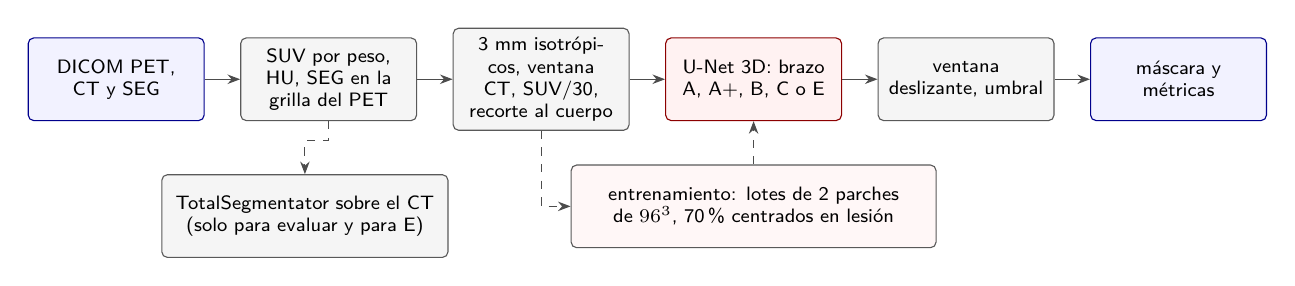
\begin{tikzpicture}[font=\sffamily\scriptsize, node distance=0.45cm,
  caja/.style={draw=black!65,fill=black!4,rounded corners=2pt,align=center,minimum height=1.05cm,text width=2.0cm},
  dato/.style={draw=blue!55!black,fill=blue!5,rounded corners=2pt,align=center,minimum height=1.05cm,text width=2.0cm},
  red/.style={draw=red!55!black,fill=red!5,rounded corners=2pt,align=center,minimum height=1.05cm,text width=2.0cm},
  fl/.style={-{Stealth[length=1.6mm]},draw=black!70}]
\node[dato] (d) {DICOM PET, CT y SEG};
\node[caja,right=of d] (c) {SUV por peso, HU, SEG en la grilla del PET};
\node[caja,right=of c] (p) {3 mm isotrópicos, ventana CT, SUV/30, recorte al cuerpo};
\node[red,right=of p] (n) {U-Net 3D: brazo A, A+, B, C o E};
\node[caja,right=of n] (s) {ventana deslizante, umbral};
\node[dato,right=of s] (m) {máscara y métricas};
\draw[fl] (d)--(c); \draw[fl] (c)--(p); \draw[fl] (p)--(n); \draw[fl] (n)--(s); \draw[fl] (s)--(m);
\node[caja,below=0.55cm of n,text width=4.4cm,fill=red!3] (t) {entrenamiento: lotes de 2 parches de $96^3$, 70\,\% centrados en lesión};
\draw[fl,dashed] (p.south) |- (t.west);
\draw[fl,dashed] (t.north) -- (n.south);
\node[caja,below=0.55cm of p,xshift=-3.0cm,text width=3.4cm] (o) {TotalSegmentator sobre el CT (solo para evaluar y para E)};
\draw[fl,dashed] (c.south) -- ++(0,-0.25) -| (o.north);
\end{tikzpicture}
\caption{Recorrido de un estudio. Las líneas discontinuas son caminos que solo se usan para entrenar o para evaluar.}
\label{fig:pipeline}
\end{figure}

\subsection{Conversión y preprocesamiento}

El SUV se calcula desde las etiquetas DICOM: actividad del vóxel, dosis inyectada corregida por decaimiento entre la inyección y la adquisición, y peso del paciente \citep{boellaard2015}. El CT se remuestrea a la grilla del PET. La máscara del DICOM SEG se ubica corte a corte por su posición física, porque el orden de los cortes en el archivo no coincide con el del PET; ese error de orientación apareció el primer día y lo corregí con una prueba sobre un fantoma sintético.

Después, todo se lleva a vóxeles isotrópicos de 3 mm. El CT se recorta a la ventana de tejido blando, de $-200$ a 300 HU, y se escala a $[0,1]$. El SUV se divide por 30 con tope en 1. Una máscara corporal, obtenida del CT, permite recortar el volumen a la caja del cuerpo: cada estudio queda en unos $284\times120\times135$ vóxeles. Todas las constantes son fijas, de modo que el preprocesamiento no aprende nada de validación ni de prueba.

\subsection{Referencia clásica}

La referencia clásica aplica un umbral de SUV $\geq 2{,}5$, una apertura morfológica de radio 1 y elimina las componentes de menos de 0,5 mL. Es la referencia que reporté en la parcial y la que aparece en todas las tablas. La definición de tema prometía además apagar los órganos de captación fisiológica; las reglas escritas a mano borraban lesiones reales, así que la variante con exclusión de órganos la calculé después con los mapas de TotalSegmentator \citep{wasserthal2023} y la reporto como análisis secundario (sección~\ref{sec:secundarios}).

\subsection{Los brazos de fusión}

Todos los brazos parten de la misma U-Net 3D de MONAI \citep{ronneberger2015,cicek2016,cardoso2022monai}, con cinco niveles de 32, 64, 128, 256 y 320 canales, unidades residuales y normalización de instancia \citep{ulyanov2016}. El codificador reduce el cubo de 96 a 6 vóxeles por lado en cuatro pasos, y el decodificador lo devuelve a 96 con conexiones de salto en cada nivel. La salida tiene dos canales, fondo y lesión, y una softmax da la probabilidad de lesión por vóxel. La Figura~\ref{fig:brazos} muestra cómo entra cada modalidad.

\begin{itemize}
\item \textbf{A, fusión temprana.} El SUV y el CT entran como dos canales de una sola red. Desde la primera convolución cada filtro mira las dos modalidades. Tiene 12,9 M parámetros y cuesta unos 37 GFLOP por parche.
\item \textbf{B, fusión intermedia por concatenación.} Cada modalidad entra con un canal a su propio codificador. En el cuello de botella los dos mapas de 320 canales se apilan en 640 y una convolución $1\times1\times1$ los combina en 320. El decodificador es uno solo y recibe las conexiones de salto de los dos codificadores. Tiene 24,0 M parámetros y cuesta unos 59 GFLOP por parche.
\item \textbf{C, B más atención cruzada} en el cuello de botella, descrita en la sección siguiente (24,4 M).
\item \textbf{E, referencia hepática.} Es A con un tercer canal: el SUV dividido por la mediana del SUV hepático del propio paciente, con tope en 8 veces. El hígado se segmenta con TotalSegmentator sobre el CT y la mediana se calcula sin mirar la anotación, para que el canal exista igual en un estudio nuevo. Lo agregué el 10 de septiembre por dos razones. La clínica ya compara la captación con el hígado del paciente en la escala de Deauville para linfoma \citep{barrington2014}. Y la red ve parches de 29 cm: desde un parche en la pelvis el hígado no se ve, así que esa referencia es un dato que el parche no contiene.
\item \textbf{A+, control de capacidad.} Es A con 1,375 veces más canales en cada nivel, para llegar a 24,3 M parámetros, como B. Lo agregué en la etapa extendida, después de una auditoría del código, para separar el efecto de tener más red del efecto de fusionar distinto.
\end{itemize}

B cumple dos papeles. Es la fusión intermedia sin atención y es el control de C: si C le gana a A pero empata con B, la ventaja es del doble codificador y no de la atención.

\begin{figure}[h]
\centering
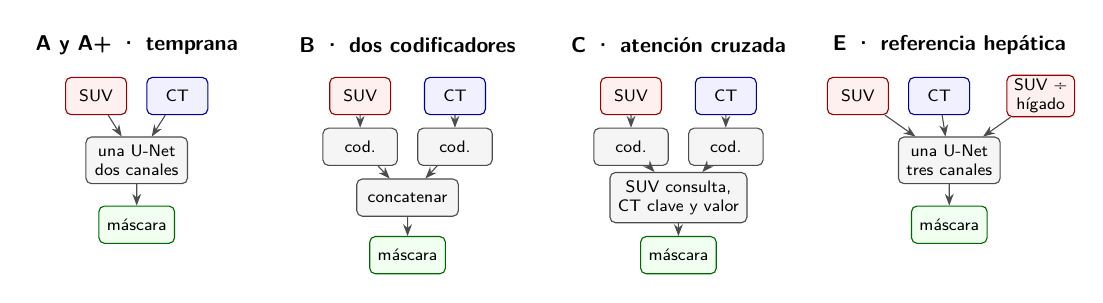
\begin{tikzpicture}[scale=0.86,transform shape,
  font=\sffamily\scriptsize,
  pet/.style={draw=red!60!black,fill=red!6,rounded corners=2pt,minimum width=0.9cm,minimum height=0.55cm},
  ct/.style={draw=blue!60!black,fill=blue!6,rounded corners=2pt,minimum width=0.9cm,minimum height=0.55cm},
  enc/.style={draw=black!70,fill=black!4,rounded corners=2pt,minimum width=1.5cm,minimum height=0.55cm,align=center},
  sal/.style={draw=green!40!black,fill=green!6,rounded corners=2pt,minimum width=1.1cm,minimum height=0.55cm},
  fl/.style={-{Stealth[length=1.5mm]},draw=black!70}]
\node[font=\sffamily\bfseries\small] at (0,1.15) {A y A+ · temprana};
\node[pet] (pa) at (-0.6,0.4) {SUV}; \node[ct] (ca) at (0.6,0.4) {CT};
\node[enc] (ea) at (0,-0.55) {una U-Net\\ dos canales};
\node[sal] (oa) at (0,-1.5) {máscara};
\draw[fl] (pa)--(ea); \draw[fl] (ca)--(ea); \draw[fl] (ea)--(oa);
\node[font=\sffamily\bfseries\small] at (4,1.15) {B · dos codificadores};
\node[pet] (pb) at (3.3,0.4) {SUV}; \node[ct] (cb) at (4.7,0.4) {CT};
\node[enc,minimum width=1.1cm] (e1) at (3.3,-0.35) {cod.}; \node[enc,minimum width=1.1cm] (e2) at (4.7,-0.35) {cod.};
\node[enc] (jb) at (4,-1.1) {concatenar};
\node[sal] (ob) at (4,-1.95) {máscara};
\draw[fl] (pb)--(e1); \draw[fl] (cb)--(e2); \draw[fl] (e1)--(jb); \draw[fl] (e2)--(jb); \draw[fl] (jb)--(ob);
\node[font=\sffamily\bfseries\small] at (8,1.15) {C · atención cruzada};
\node[pet] (pc) at (7.3,0.4) {SUV}; \node[ct] (cc) at (8.7,0.4) {CT};
\node[enc,minimum width=1.1cm] (e3) at (7.3,-0.35) {cod.}; \node[enc,minimum width=1.1cm] (e4) at (8.7,-0.35) {cod.};
\node[enc] (jc) at (8,-1.1) {SUV consulta,\\ CT clave y valor};
\node[sal] (oc) at (8,-1.95) {máscara};
\draw[fl] (pc)--(e3); \draw[fl] (cc)--(e4); \draw[fl] (e3)--(jc); \draw[fl] (e4)--(jc); \draw[fl] (jc)--(oc);
\node[font=\sffamily\bfseries\small] at (12,1.15) {E · referencia hepática};
\node[pet] (pe) at (10.65,0.4) {SUV}; \node[ct] (ce) at (11.85,0.4) {CT};
\node[pet,minimum width=1.0cm,align=center,inner sep=1.5pt] (he) at (13.35,0.4) {SUV ÷\\ hígado};
\node[enc] (ee) at (12,-0.55) {una U-Net\\ tres canales};
\node[sal] (oe) at (12,-1.5) {máscara};
\draw[fl] (pe)--(ee); \draw[fl] (ce)--(ee); \draw[fl] (he)--(ee); \draw[fl] (ee)--(oe);
\end{tikzpicture}
\caption{Los brazos. En B y C cada modalidad tiene su propio codificador y se unen en el cuello de botella ($6^3$ posiciones). A+ tiene la forma de A con 1,375 veces más canales.}
\label{fig:brazos}
\end{figure}

\subsection{La atención cruzada del brazo C}

En el cuello de botella, cada codificador entrega un mapa de 320 canales sobre una grilla de $6\times6\times6$: 216 posiciones, cada una de las cuales resume unos 48 mm del parche. C deja que cada posición del PET busque, entre las 216 posiciones del CT, las que le sirven \citep{vaswani2017}. Con $X_P, X_C \in \mathbb{R}^{216\times320}$ los mapas aplanados del PET y del CT, $\mathrm{LN}$ una normalización de capa y $E$ una codificación de posición sinusoidal 3D fija,
\begin{align}
Q &= (\mathrm{LN}(X_P)+E)\,W_Q, \\
K &= (\mathrm{LN}(X_C)+E)\,W_K, \qquad V = (\mathrm{LN}(X_C)+E)\,W_V, \\
\mathrm{Att}(Q,K,V) &= \mathrm{softmax}\!\left(\frac{QK^\top}{\sqrt{d}}\right) V, \\
\tilde X_P &= X_P + \gamma\,\mathrm{MHA}(Q,K,V),
\end{align}
donde MHA son 8 cabezas de atención en paralelo y $\gamma$ es un escalar aprendido. Después, $\tilde X_P$ y $X_C$ se concatenan y siguen el mismo camino que en B.

La atención va en el cuello porque compara todas las posiciones contra todas. En $6^3$ son $216^2$ comparaciones; en $96^3$ serían $884\,736^2$, imposible en 24 GB. Estas 216 posiciones son lo más parecido, dentro de este proyecto, a los tokens de un Vision Transformer \citep{dosovitskiy2021,hatamizadeh2022}, con la diferencia de que salen de las convoluciones del codificador y no de cortar la imagen en baldosas.

La primera versión de C partió con $\gamma=0$, para que naciera igual a B y aprendiera a usar la atención si le servía. Como $\gamma$ terminó en 0,0125, la reentrené con $\gamma=1$, para que la atención participara con todo su peso desde el inicio.

\subsection{Entrenamiento por parches}

Un estudio de cuerpo entero tiene unos 4,6 millones de vóxeles por canal, y con todos los mapas intermedios de la U-Net no cabe en la memoria del equipo. La red aprende con parches de $96^3$ vóxeles, 288 mm de lado. Como la lesión ocupa menos del 1\,\% del cuerpo, el 70\,\% de los parches se centra en un vóxel de lesión y el resto en cualquier vóxel del cuerpo. El Algoritmo~\ref{alg:entrenar} resume una corrida.

\begin{algorithm}[h]
\caption{Una corrida de entrenamiento (igual para todos los brazos).}
\label{alg:entrenar}
\small
\begin{algorithmic}[1]
\Require estudios de entrenamiento $\mathcal{D}$, red $f_\theta$, iteraciones $T$ (25\,000 o 100\,000)
\For{$t = 1$ \textbf{hasta} $T$}
  \State tomar 2 estudios de $\mathcal{D}$ y recortar de cada uno un cubo de $96^3$ (70\,\% centrado en lesión)
  \State voltear al azar izquierda-derecha y adelante-atrás, con la máscara incluida; nunca cabeza-pies
  \State $\hat y \gets \mathrm{softmax}(f_\theta(x))$ \Comment{$x$: $[2, C, 96, 96, 96]$, con $C=2$ o 3 canales}
  \State $\mathcal{L} \gets \mathcal{L}_{\mathrm{Dice}}(\hat y, y) + \mathcal{L}_{\mathrm{CE}}(\hat y, y)$
  \State gradientes por retropropagación, recortados a norma 12
  \State AdamW: $\theta \gets \theta - \eta_t \cdot \mathrm{paso}$, con $\eta_t = 3\cdot10^{-4}(1-t/T)^{0{,}9}$
  \If{$t \bmod 500 = 0$} guardar \texttt{ultimo.pt} \EndIf
  \If{$t \bmod 1000 = 0$} Dice en 12 estudios fijos de validación; si es el mejor, guardar \texttt{mejor.pt} \EndIf
\EndFor
\end{algorithmic}
\end{algorithm}

El lote es de 2 parches por memoria: dos cubos 3D de este tamaño caben con margen en 24 GB, y nnU-Net usa el mismo lote en 3D \citep{isensee2021nnunet}. La pérdida combina Dice, que mira el solapamiento global y no se deja dominar por el fondo, y entropía cruzada, que corrige cada vóxel. El optimizador es AdamW \citep{loshchilov2019} con decaimiento de pesos $10^{-5}$.

\subsection{Inferencia y sistema final}

Para predecir un estudio, la red lo recorre con cubos de $96^3$ que se solapan a la mitad y promedia las probabilidades de cada vóxel con más peso en el centro de cada cubo (ponderación gaussiana), porque en el borde la red ve menos contexto.

El sistema final agrega dos cosas sobre B. Primero, un ensamble: los 825 estudios de entrenamiento se dividieron en cinco pliegues estratificados de unos 165, y entrené cinco modelos B, cada uno con cuatro pliegues. Segundo, aumento en inferencia (TTA): cada modelo predice también la imagen volteada de izquierda a derecha, de adelante hacia atrás y en los dos sentidos a la vez, y se devuelve cada volteo antes de promediar. El umbral de decisión se fijó en 0,6 con una regla escrita antes de abrir la prueba (sección~\ref{sec:umbral}). El Algoritmo~\ref{alg:final} lo resume.

\begin{algorithm}[h]
\caption{Predicción del sistema final para un estudio.}
\label{alg:final}
\small
\begin{algorithmic}[1]
\Require estudio preprocesado $x$, modelos $f_1,\dots,f_5$ (B, uno por pliegue), volteos $\mathcal{V} = \{\mathrm{id}, v_1, v_2, v_3\}$
\State $P \gets 0$
\For{$k = 1$ \textbf{hasta} 5}
  \For{\textbf{cada} $v \in \mathcal{V}$}
    \State $P \gets P + v^{-1}\big(\mathrm{VentanaDeslizante}(f_k, v(x))\big)$ \Comment{cubos de $96^3$, solape 50\,\%}
  \EndFor
\EndFor
\State $P \gets P / 20$ \Comment{20 lecturas por estudio}
\Ensure máscara $M = [P \geq 0{,}6]$
\end{algorithmic}
\end{algorithm}

\section{Implementación}

\subsection{Organización del repositorio}

El código está en Python y separa una biblioteca, \texttt{src/petct}, de los scripts numerados que la usan en el orden del proyecto. La biblioteca no conoce los datos de ningún estudio en particular; los scripts leen un manifiesto, llaman a la biblioteca y escriben tablas en \texttt{results/} y figuras en \texttt{docs/figuras/}. La Tabla~\ref{tab:modulos} resume los módulos.

\begin{table}[h]
\centering\small
\caption{Módulos de \texttt{src/petct}.}
\label{tab:modulos}
\begin{tabularx}{\linewidth}{@{}lX@{}}
\toprule
Módulo & Qué hace \\
\midrule
\texttt{suv.py}, \texttt{convert.py}, \texttt{geometry.py} & SUV por peso desde DICOM con corrección de decaimiento; DICOM a NIfTI; CT a la grilla del PET; DICOM SEG ubicado por posición física. \\
\texttt{tcia.py} & Selección estratificada y reproducible del subconjunto; descarga desde TCIA. \\
\texttt{preprocess.py}, \texttt{data.py} & Remuestreo, ventana, escalado, máscara corporal, recorte; muestreo de parches con sesgo a lesión y volteos. \\
\texttt{classical.py} & Referencia clásica: umbral, apertura, tamaño mínimo y exclusión opcional de órganos. \\
\texttt{models.py} & Los brazos A, A+, B, C y E sobre bloques de MONAI; atención cruzada con codificación de posición 3D. \\
\texttt{losses.py}, \texttt{train.py}, \texttt{device.py} & Dice más entropía cruzada (con peso opcional por órgano); bucle de entrenamiento con checkpoints; selección del acelerador. \\
\texttt{infer.py}, \texttt{postproc.py} & Ventana deslizante con ponderación gaussiana y TTA; reglas de posproceso. \\
\texttt{metrics.py}, \texttt{organs.py} & Dice, FPV y FNV por componentes 26-conexas; zona anonimizada; reparto de errores por órgano con TotalSegmentator. \\
\texttt{reference.py} & Referencia hepática del paciente para el brazo E. \\
\bottomrule
\end{tabularx}
\end{table}

Los scripts siguen el orden de trabajo: 01 a 04 seleccionan, descargan, convierten y preprocesan; 05 es la referencia clásica; 07 entrena; 09 evalúa y guarda máscaras; 11 a 20 son los análisis del acto 1; 24 a 39 son la etapa extendida, el ensamble, la decisión del umbral y la prueba; 40 a 43 son los análisis secundarios, los casos y el falso positivo por órgano de todos los brazos. Las pruebas de \texttt{tests/} cubren el cálculo del SUV, la geometría con un fantoma sintético, el preprocesamiento, la forma de las salidas de los modelos y el reparto por órgano.

\subsection{Decisiones de diseño}

\textbf{Un solo equipo, sin GPU de servidor.} Todo se entrenó en un MacBook Pro con chip M5 y 24 GB de memoria compartida, con el acelerador \texttt{mps} de PyTorch en precisión simple. A tarda 0,65 s por iteración y B y C 0,79 s: entre 4,8 y 6,5 horas por corrida de 25\,000 iteraciones y cerca de un día por corrida de 100\,000. En total hice 38 corridas de entrenamiento. Este límite explica el tamaño de los parches, el lote de 2 y que la atención vaya solo en el cuello.

\textbf{Reproducibilidad y fugas.} La partición es por paciente y se guarda como manifiesto con su md5. El preprocesamiento usa constantes fijas. El 6 de septiembre congelé el protocolo de entrenamiento (\texttt{docs/PROTOCOLO\_CONGELADO.md}) y audité las fugas: ningún paciente en dos particiones, ninguna estadística calculada sobre validación o prueba. TotalSegmentator y la referencia hepática se calculan solo desde el CT y el PET, sin la anotación.

\textbf{Una prueba con candado.} Antes de abrir la prueba escribí y versioné en git las hipótesis, los brazos, los checkpoints, el umbral y los criterios de confirmación (\texttt{docs/TEST\_PREREGISTRO.md}). El script de la prueba se niega a correr si esos archivos tienen cambios sin registrar, y deja un acta con la hora y el commit de apertura. La abrí una sola vez, el 12 de octubre.

\textbf{Métricas propias contrastadas.} Implementé Dice, FPV y FNV con las definiciones del reto y las contrasté al final con el script oficial \citep{labmidas}, copiado sin cambios en \texttt{scripts/oficial\_autopet/} (sección~\ref{sec:secundarios}).

\textbf{Datos fuera del repositorio.} La colección completa en DICOM pesa cerca de 419 GB y cada estudio preprocesado unos 12 MB. Ninguno se sube a git; el README explica cómo descargarlos y regenerarlos con los scripts.

\section{Metodología experimental}

\subsection{Diseño en dos etapas}

\textbf{Acto 1} (3 al 12 de septiembre, rama \texttt{main}). Los cuatro brazos de la definición y de la parcial (A, B, C y E), cada uno con tres semillas (423, 2 y 3), 176 estudios de entrenamiento, 25\,000 iteraciones y el checkpoint \texttt{mejor.pt}. Es lo que reportó la entrega parcial.

\textbf{Etapa extendida} (12 de septiembre al 12 de octubre, rama \texttt{extendido}). El empate del acto 1 dejó abierta una pregunta: si las arquitecturas son equivalentes o si el montaje no les dio con qué separarse. La etapa extendida la abordó en cuatro pasos, cada uno con su criterio de éxito escrito antes de correr:
\begin{enumerate}
\item un diseño 2\,×\,2 con el brazo A: 176 o 825 estudios por 25\,000 o 100\,000 iteraciones;
\item los brazos A, A+, B y C con 825 estudios y 100\,000 iteraciones, tres semillas cada uno;
\item dos intentos de enseñar anatomía a B: preentrenar el codificador del CT para segmentar 17 grupos de órganos usando TotalSegmentator como profesor, y una pérdida que cobra tres veces más por marcar tumor dentro de un órgano de captación fisiológica;
\item el ensamble de cinco pliegues con TTA, con predicción fuera de pliegue para los 825 estudios.
\end{enumerate}
En esta etapa usé siempre \texttt{ultimo.pt}, por lo que encontré en el acto 1 sobre el criterio de checkpoint. Validación y prueba siguieron exactamente iguales; los estudios nuevos entraron solo a entrenamiento.

\subsection{Métricas}

Por estudio calculo, con componentes 26-conexas y en la métrica corregida:
\begin{itemize}
\item \textbf{\dmas}: el Dice entre predicción y verdad, promediado solo en los estudios con lesión. En un control el Dice no está definido.
\item \textbf{FPV}: mililitros de las componentes predichas que no tocan ninguna lesión anotada. Mide lo que el modelo inventa donde no hay nada.
\item \textbf{FNV}: mililitros de las lesiones anotadas que no toca ninguna componente predicha.
\item \textbf{Detección por lesión} según tamaño y \textbf{marcas falsas por estudio}, que traducen el FPV al trabajo de un médico que corrige la máscara.
\item \textbf{FP por órgano}: el FPV repartido según el mapa de órganos de TotalSegmentator \citep{wasserthal2023}.
\item Como análisis secundarios: Hausdorff 95 \citep{maierhein2024}, error de SUVmax por paciente y contraste con el script oficial.
\end{itemize}

\subsection{Estadística}

Las comparaciones son pareadas por estudio: para cada estudio se calcula la diferencia entre dos brazos y se analiza esa lista, lo que quita la variación entre pacientes. Con varias semillas, primero promedio el brazo por estudio. El intervalo de confianza del 95\,\% de la diferencia media sale de un bootstrap de 10\,000 remuestreos de estudios con semilla 423 \citep{efron1993}. Reporto además la prueba de rangos con signo de Wilcoxon y en cuántos estudios gana cada brazo. Una diferencia cuyo intervalo cruza el cero la leo como no demostrada, no como igualdad.

\subsection{Preregistro de la prueba}
\label{sec:umbral}

Antes de abrir la prueba fijé dos hipótesis, ambas contra B extendido con sus tres semillas:
\begin{itemize}
\item \textbf{H1.} El ensamble de cinco pliegues con TTA, a umbral 0,5, mejora a B.
\item \textbf{H2.} El sistema final, ensamble con TTA al umbral y con la regla de posproceso decididos sin la prueba, mejora a B.
\end{itemize}
Cada una se confirma solo si el IC95 de $\Delta$\dmas{} queda entero sobre cero \emph{y} el IC95 de $\Delta$FPV queda entero bajo cero. Las demás comparaciones (acto 1, arquitecturas del extendido, preentrenamiento, umbral 0,7, métrica cruda) quedaron declaradas como secundarias, S1 a S8.

El umbral y una regla del hígado (borrar islas cuyo SUVmax no llegue al doble del hígado del paciente) se decidieron con los 825 estudios predichos fuera de pliegue y con reglas escritas antes de ver los números. Para el umbral, el de mayor \dmas{} entre los que pierden como máximo 2 puntos porcentuales de lesiones detectadas respecto de 0,5. Para la regla del hígado, adoptarla solo si baja las marcas falsas al menos un 25\,\%, pierde como máximo el 3\,\% de las lesiones detectadas y no baja el \dmas{} más de 0,005.

\section{Resultados}

\subsection{Acto 1: las fusiones empatan en validación}

La Tabla~\ref{tab:acto1} repite la tabla de la entrega parcial. Frente a A, la diferencia pareada de \dmas{} es $-0{,}009$ para B (IC95 $-0{,}055$ a $+0{,}024$; $p=0{,}52$), $-0{,}009$ para C ($-0{,}061$ a $+0{,}030$; $p=0{,}87$) y $+0{,}018$ para E ($-0{,}020$ a $+0{,}062$; $p=0{,}93$). Los tres intervalos cruzan el cero. Todas las redes, en cambio, dejan 57 veces menos falso positivo que el umbral clásico, con un \dmas{} tres veces y media mayor. Por diagnóstico, el patrón se repite en todos los brazos: pulmón cerca de 0,74, linfoma 0,70 y melanoma 0,40.

\begin{table}[h]
\centering\small
\caption{Acto 1, validación (26 estudios, 20 positivos evaluables). Media $\pm$ desviación entre tres semillas. \texttt{mejor.pt} es el checkpoint del protocolo; \texttt{ultimo.pt}, la iteración 25\,000.}
\label{tab:acto1}
\begin{tabular}{lcccccc}
\toprule
 & \multicolumn{3}{c}{\texttt{mejor.pt}} & \multicolumn{3}{c}{\texttt{ultimo.pt}} \\
\cmidrule(lr){2-4}\cmidrule(lr){5-7}
Brazo & \dmas & FPV (mL) & FNV (mL) & \dmas & FPV (mL) & FNV (mL) \\
\midrule
A & 0,621 $\pm$ 0,016 & 20,9 $\pm$ 2,5 & 6,0 & 0,615 $\pm$ 0,020 & 21,7 $\pm$ 0,5 & 5,9 \\
B & 0,612 $\pm$ 0,014 & 22,8 $\pm$ 3,1 & 5,4 & 0,607 $\pm$ 0,002 & 22,1 $\pm$ 2,8 & 4,4 \\
C & 0,612 $\pm$ 0,008 & 23,2 $\pm$ 6,7 & 5,9 & 0,610 $\pm$ 0,007 & 21,5 $\pm$ 1,8 & 4,5 \\
E & 0,640 $\pm$ 0,022 & 22,0 $\pm$ 9,8 & 7,3 & 0,638 $\pm$ 0,006 & 23,6 $\pm$ 2,8 & 5,7 \\
Clásica & 0,180 & 1\,191,9 & 5,6 & & & \\
\bottomrule
\end{tabular}
\end{table}

\textbf{La atención de C quedó inerte.} Al forzar $\gamma=0$ en el modelo entrenado, la predicción no cambió en un solo vóxel: diferencia de Dice 0,000 en los 26 estudios y en las tres semillas. Medí por qué. Los pesos de atención resultaron casi uniformes sobre las 216 posiciones, de modo que cada posición del PET recibía casi el mismo vector, un promedio de todo el CT. La salida de la atención era en un 99\,\% constante en el espacio. La convolución que sigue tiene normalización de instancia, que resta a cada canal su media espacial, y una señal igual en todas las posiciones desaparece.

\textbf{El canal de E está vivo, pero no paga.} Al reemplazar la referencia hepática del paciente por una constante poblacional (2,165, la mediana de los 176 de entrenamiento), cambian 23 de 26 predicciones, pero el efecto neto sobre el FPV es de 1,4 mL, menor que la variación entre semillas. Su ventaja aparente venía del checkpoint: el protocolo había elegido la iteración 9\,000.

\textbf{El checkpoint pesa más que la semilla.} \texttt{mejor.pt} se elige con el máximo Dice de una validación rápida de 12 estudios, una curva muy ruidosa (Figura~\ref{fig:curvas}). Al usar el checkpoint final, la desviación del FPV entre semillas baja 5,1 veces en A, 3,8 en C y 3,4 en E, mientras el Dice medio cambia 0,005 y el orden entre modelos se mantiene. Elegir el máximo de una curva ruidosa optimiza una métrica y deja las otras al azar.

\begin{figure}[h]
\centering
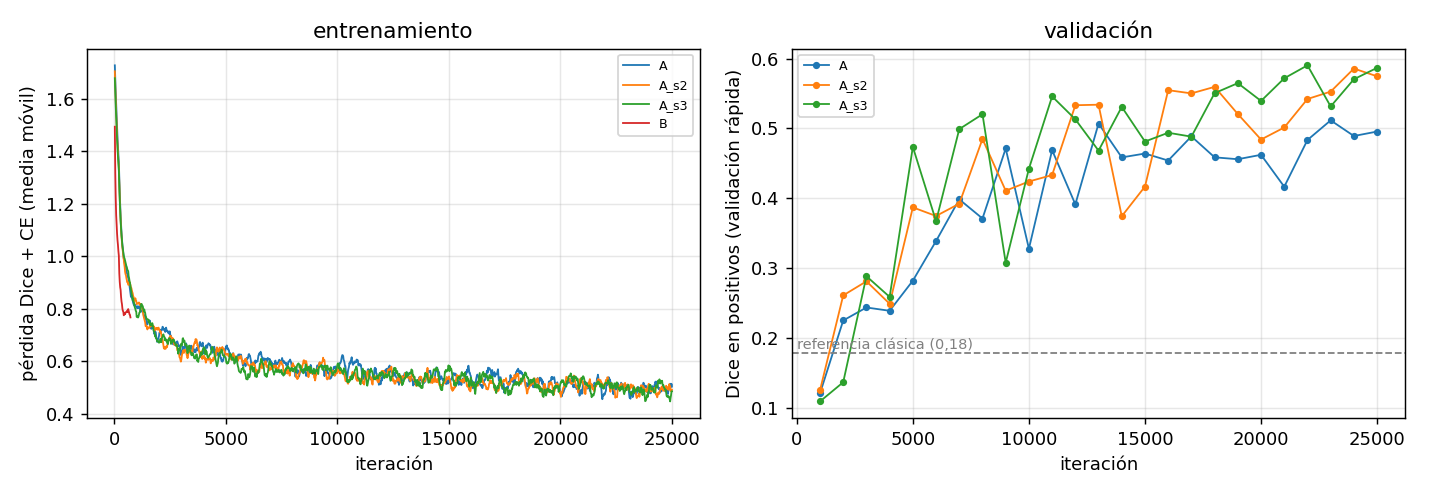
\includegraphics[width=\linewidth]{curvas_entrenamiento.png}
\caption{Acto 1: pérdida de entrenamiento (izquierda) y Dice de la validación rápida de 12 estudios (derecha) en las doce corridas. La pérdida baja igual en todos los brazos. La curva de validación salta de un punto a otro, y elegir su máximo como checkpoint introduce ruido en el falso positivo.}
\label{fig:curvas}
\end{figure}

\subsection{Etapa extendida: el empate era falta de entrenamiento}

\textbf{Paso 1, datos o tiempo.} Cuadruplicar las iteraciones mejoró el \dmas{} de A en +0,041 y +0,045, ganando en 17 de 20 estudios las dos veces (Tabla~\ref{tab:2x2}). Quintuplicar los estudios con las iteraciones fijas no movió nada claro: con 25\,000 iteraciones y 825 estudios, cada estudio se veía en promedio 61 veces en vez de 284. El cuello de botella del acto 1 era cuánto entrenaba la red.

\begin{table}[h]
\centering\small
\caption{Paso 1, diseño 2\,×\,2 con el brazo A (validación, una semilla).}
\label{tab:2x2}
\begin{tabular}{lccc}
\toprule
 & \dmas & FPV (mL) & FNV (mL) \\
\midrule
176 estudios, 25\,000 iteraciones & 0,615 & 21,7 & 5,9 \\
176 estudios, 100\,000 iteraciones & 0,655 & 15,5 & 5,2 \\
825 estudios, 25\,000 iteraciones & 0,636 & 24,7 & 5,1 \\
825 estudios, 100\,000 iteraciones & 0,681 & 15,8 & 3,9 \\
\bottomrule
\end{tabular}
\end{table}

\textbf{Paso 2, las arquitecturas con entrenamiento suficiente.} Con 825 estudios y 100\,000 iteraciones, los brazos de doble codificador quedaron arriba (Tabla~\ref{tab:paso2}): el orden del acto 1 se invirtió. A+, con los mismos parámetros que B, empató con A. En validación, con 20 positivos, la ventaja de B sobre A con tres semillas fue de +0,012, con un intervalo que cruzaba el cero. La atención de C siguió inerte: $\gamma$ terminó en 0,992 y la ablación volvió a dar cero en las tres semillas.

\begin{table}[h]
\centering\small
\caption{Paso 2, validación, 825 estudios y 100\,000 iteraciones, media de tres semillas.}
\label{tab:paso2}
\begin{tabular}{lccc}
\toprule
Brazo & Parámetros & \dmas & FPV (mL) \\
\midrule
A & 12,9 M & 0,694 & 15,1 \\
A+ & 24,3 M & 0,694 & 15,8 \\
B & 24,0 M & 0,705 & 13,3 \\
C & 24,4 M & 0,713 & 13,2 \\
\bottomrule
\end{tabular}
\end{table}

\textbf{Paso 3, enseñar anatomía no cumplió sus criterios.} Con B, el falso positivo en órganos fisiológicos ya era solo el 18\,\% del total; el resto estaba en tejido sin etiqueta, pulmón y bordes. El codificador del CT preentrenado aprendió los 17 grupos de órganos con un Dice anatómico de 0,861, y B partiendo de él dio con una semilla el mejor Dice de todas las corridas largas, 0,724. Antes de correr más declaré una hipótesis nueva: aceptarlo solo si las semillas 2 y 3 daban ambas 0,716 o más. Dieron 0,700 y 0,698. Con tres semillas, B preentrenada quedó en 0,707 frente a 0,705 de B ($p=0{,}78$). La pérdida pesada por órgano tampoco cumplió su criterio.

\textbf{Paso 4, el ensamble.} En validación, B solo dio \dmas{} 0,706 y 13,3 mL de FPV; el ensamble, 0,744 y 10,0 mL; el ensamble con TTA, 0,754 y 9,2 mL. El criterio fijado antes era FPV menor que 9 mL y no se cumplió, pero contra B la mejora fue significativa en Dice (+0,048, IC95 +0,024 a +0,079) y en FPV ($-4{,}0$ mL, IC95 $-6{,}6$ a $-2{,}2$). Detectó las mismas lesiones que B (160 de 256) con la mitad de marcas falsas por estudio (2,8 contra 4,8 a 5,8). La predicción fuera de pliegue de los 825 estudios dio \dmas{} 0,689, la primera medición del proyecto sobre más de 26 estudios.

\textbf{El umbral y la regla del hígado.} En los 825 estudios fuera de pliegue el \dmas{} era casi plano entre umbrales (0,698 a 0,699), mientras en los 26 de validación subía de 0,754 a 0,784 entre 0,5 y 0,7: esa subida era ruido de 26 estudios. La regla eligió 0,6. La regla del hígado bajó las marcas falsas un 22\,\% y perdió el 6,4\,\% de las lesiones, así que no se adoptó.

\subsection{La prueba}

\textbf{Las dos hipótesis se confirman} (Tabla~\ref{tab:h}). El falso positivo baja en los 49 estudios, sin excepción. El sistema final queda en \dmas{} 0,727 (mediana 0,806), FPV 9,5 mL y FNV 3,95 mL; con la métrica cruda del reto, en \dmas{} 0,705 y FPV 9,5 mL. Por diagnóstico, su \dmas{} medio es 0,721 en pulmón, 0,749 en linfoma y 0,709 en melanoma.

\begin{table}[h]
\centering\small
\caption{Hipótesis preregistradas, prueba (49 estudios, 38 positivos). Diferencias pareadas contra B extendido (media de tres semillas).}
\label{tab:h}
\begin{tabular}{lcccc}
\toprule
 & $\Delta$\dmas & IC95 & $\Delta$FPV (mL) & IC95 \\
\midrule
H1, ensamble + TTA, umbral 0,5 & +0,028 & +0,011 a +0,048 & $-7{,}0$ & $-12{,}4$ a $-3{,}4$ \\
H2, sistema final, umbral 0,6 & +0,029 & +0,006 a +0,054 & $-9{,}4$ & $-16{,}4$ a $-4{,}5$ \\
\bottomrule
\end{tabular}
\end{table}

La Tabla~\ref{tab:prueba} muestra todos los brazos. Tres lecturas:
\begin{itemize}
\item \textbf{El acto 1 se sostiene en Dice.} B, C y E contra A tienen intervalos que cruzan el cero. En FPV, B y C bajan la media de A unos 14 mL con intervalos que no cruzan el cero, pero Wilcoxon no sale significativo y el FPV baja en menos de la mitad de los estudios. La media de A (38,4 mL, mediana 13,2) la arrastran cuatro estudios donde marcó más de 200 mL. Los dos codificadores evitan algunos fallos grandes de la fusión temprana, pero no mejoran el estudio típico, y como B lo hace igual que C, nada de esto se puede atribuir a la atención.
\item \textbf{Con entrenamiento suficiente, la fusión intermedia gana.} En el extendido, B supera a A en \dmas{} (+0,038, IC95 +0,006 a +0,076) y en FPV ($-7{,}7$ mL, IC95 $-16{,}9$ a $-1{,}6$), y C hace lo mismo (+0,034 y $-7{,}6$ mL). A+ no se distingue de A (+0,001, IC95 $-0{,}007$ a $+0{,}009$). La ventaja no es por tamaño. Lo que en validación no alcanzaba a verse con 20 positivos se ve con 38.
\item \textbf{El ensamble es la mejora más grande y más sólida.} Contra sus propios cinco miembros, el ensamble con TTA gana +0,029 (IC95 +0,019 a +0,041) en 34 de 38 positivos.
\end{itemize}

\begin{table}[h]
\centering\small
\caption{Todos los brazos en la prueba, métrica corregida. Media de tres semillas salvo donde se indica.}
\label{tab:prueba}
\begin{tabular}{lccccc}
\toprule
Brazo & \dmas & mediana & FPV (mL) & FNV (mL) & FPV en controles \\
\midrule
Clásica (SUV $\geq 2{,}5$) & 0,182 & 0,128 & 832,5 & 2,1 & 987,1 \\
\addlinespace
Acto 1 · A & 0,616 & 0,664 & 38,4 & 5,8 & 85,7 \\
Acto 1 · B & 0,630 & 0,676 & 23,6 & 5,5 & 45,0 \\
Acto 1 · C & 0,607 & 0,633 & 24,8 & 6,9 & 48,5 \\
Acto 1 · E & 0,596 & 0,644 & 28,6 & 8,8 & 58,4 \\
\addlinespace
Extendido · A & 0,660 & 0,717 & 26,6 & 3,6 & 39,6 \\
Extendido · A+ & 0,662 & 0,714 & 23,5 & 4,6 & 39,4 \\
Extendido · B & 0,698 & 0,742 & 18,9 & 2,7 & 29,1 \\
Extendido · C & 0,695 & 0,734 & 18,9 & 2,6 & 29,3 \\
Extendido · B preentrenada & 0,709 & 0,758 & 16,3 & 3,1 & 25,7 \\
\addlinespace
Ensamble + TTA, umbral 0,5 (H1) & 0,726 & 0,798 & 11,9 & 3,5 & 13,8 \\
\textbf{Sistema final, umbral 0,6 (H2)} & \textbf{0,727} & \textbf{0,806} & \textbf{9,5} & \textbf{3,95} & \textbf{9,6} \\
\bottomrule
\end{tabular}
\end{table}

\textbf{Dónde queda el error.} La Figura~\ref{fig:fporg} reparte el falso positivo por órgano. El umbral clásico pone su error en órganos de captación fisiológica: hígado 167, riñones 111, vejiga 110, corazón 107 e intestino 90 mL por estudio. Las redes dejan menos de 1 mL en hígado, riñones, vejiga y corazón. Lo que les queda está en tejido sin órgano asignado, hueso, bazo y el borde del cuerpo, y el sistema final baja cada uno de esos grupos a menos de 3 mL.

\begin{figure}[h]
\centering
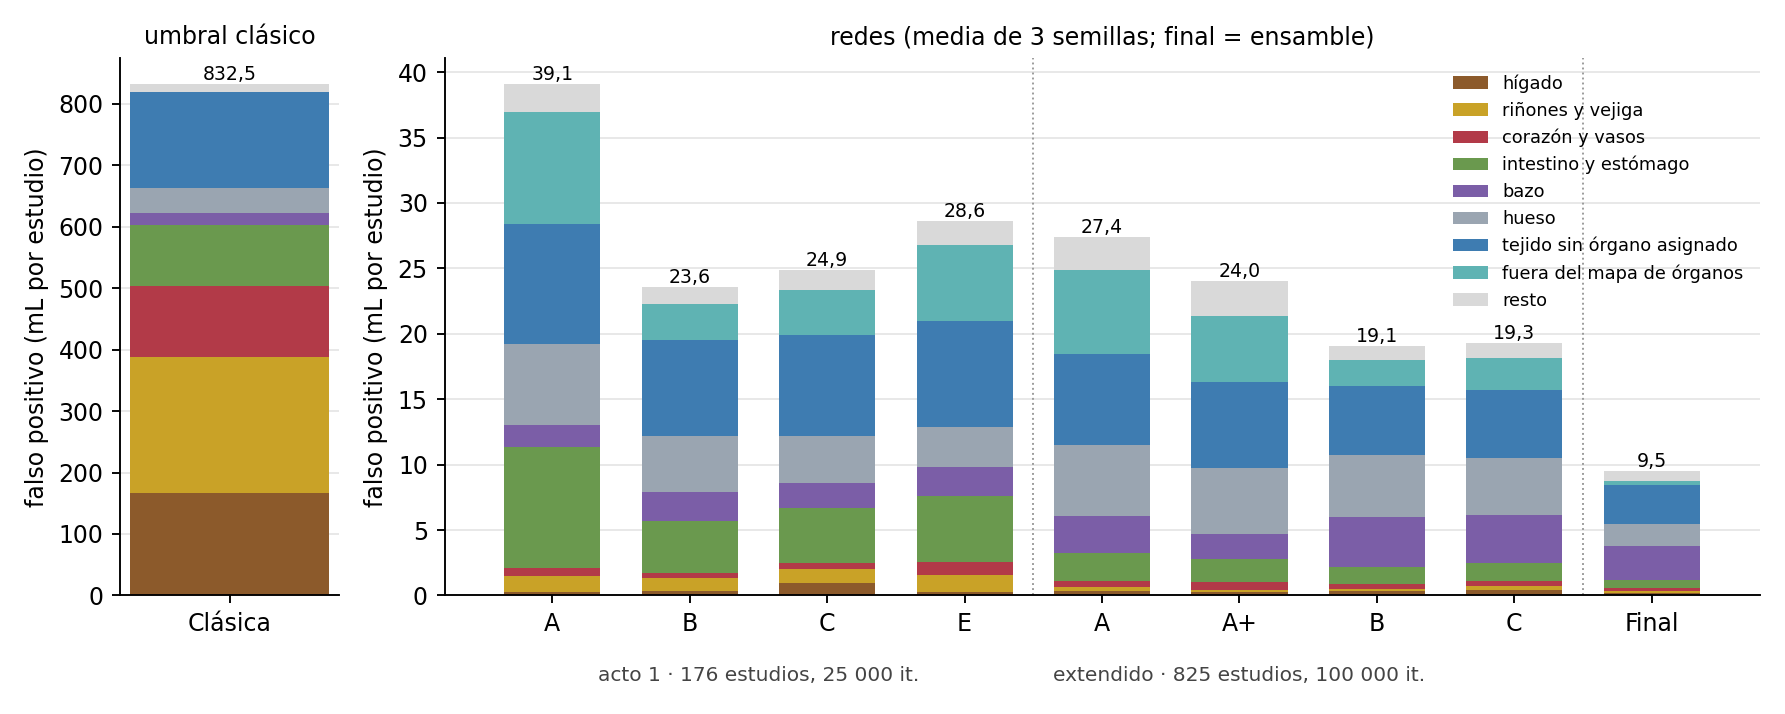
\includegraphics[width=\linewidth]{fp_por_organo_test.png}
\caption{Falso positivo por órgano en la prueba (mL por estudio, incluida la zona anonimizada, por eso A del acto 1 suma 39,1 y no 38,4). Izquierda, el umbral clásico en su propia escala; derecha, las redes. Los grupos vienen del mapa de órganos de TotalSegmentator sobre el CT.}
\label{fig:fporg}
\end{figure}

\textbf{Por lesión.} De las 435 lesiones de la prueba, el ensamble detecta 330, lo mismo que un B solo (327 a 337), con 7,8 marcas falsas por estudio en vez de 12,8 a 13,6. El sistema final baja a 6,3 marcas a cambio de 8 lesiones menos (322). Se detectan casi todas las lesiones de más de 10 mL y la mitad de las de menos de 1 mL.

\textbf{Casos.} La Figura~\ref{fig:casos} muestra cuatro estudios de la prueba elegidos con una regla fija, escrita antes de mirar las imágenes, sobre las métricas del sistema final: el caso típico (Dice más cercano a la mediana), el de mayor FPV, el de mayor FNV y el de mayor corrección del ensamble frente a B. En el caso típico (A), el umbral clásico pinta la columna, la médula y la vejiga, y las redes no. En el de mayor FPV (B), un linfoma, el error de las redes cae sobre todo en el bazo, donde la captación puede ser enfermedad no anotada. En el de mayor FNV (C), el sistema final pierde varias lesiones pequeñas que B sí tocaba: 26,0 contra 8,8 mL, el costo del umbral 0,6 visto en un paciente. En el control (D), el ensamble baja el FPV de B de 171 a 66 mL, y lo que queda está en la pelvis.

\begin{figure}[p]
\centering
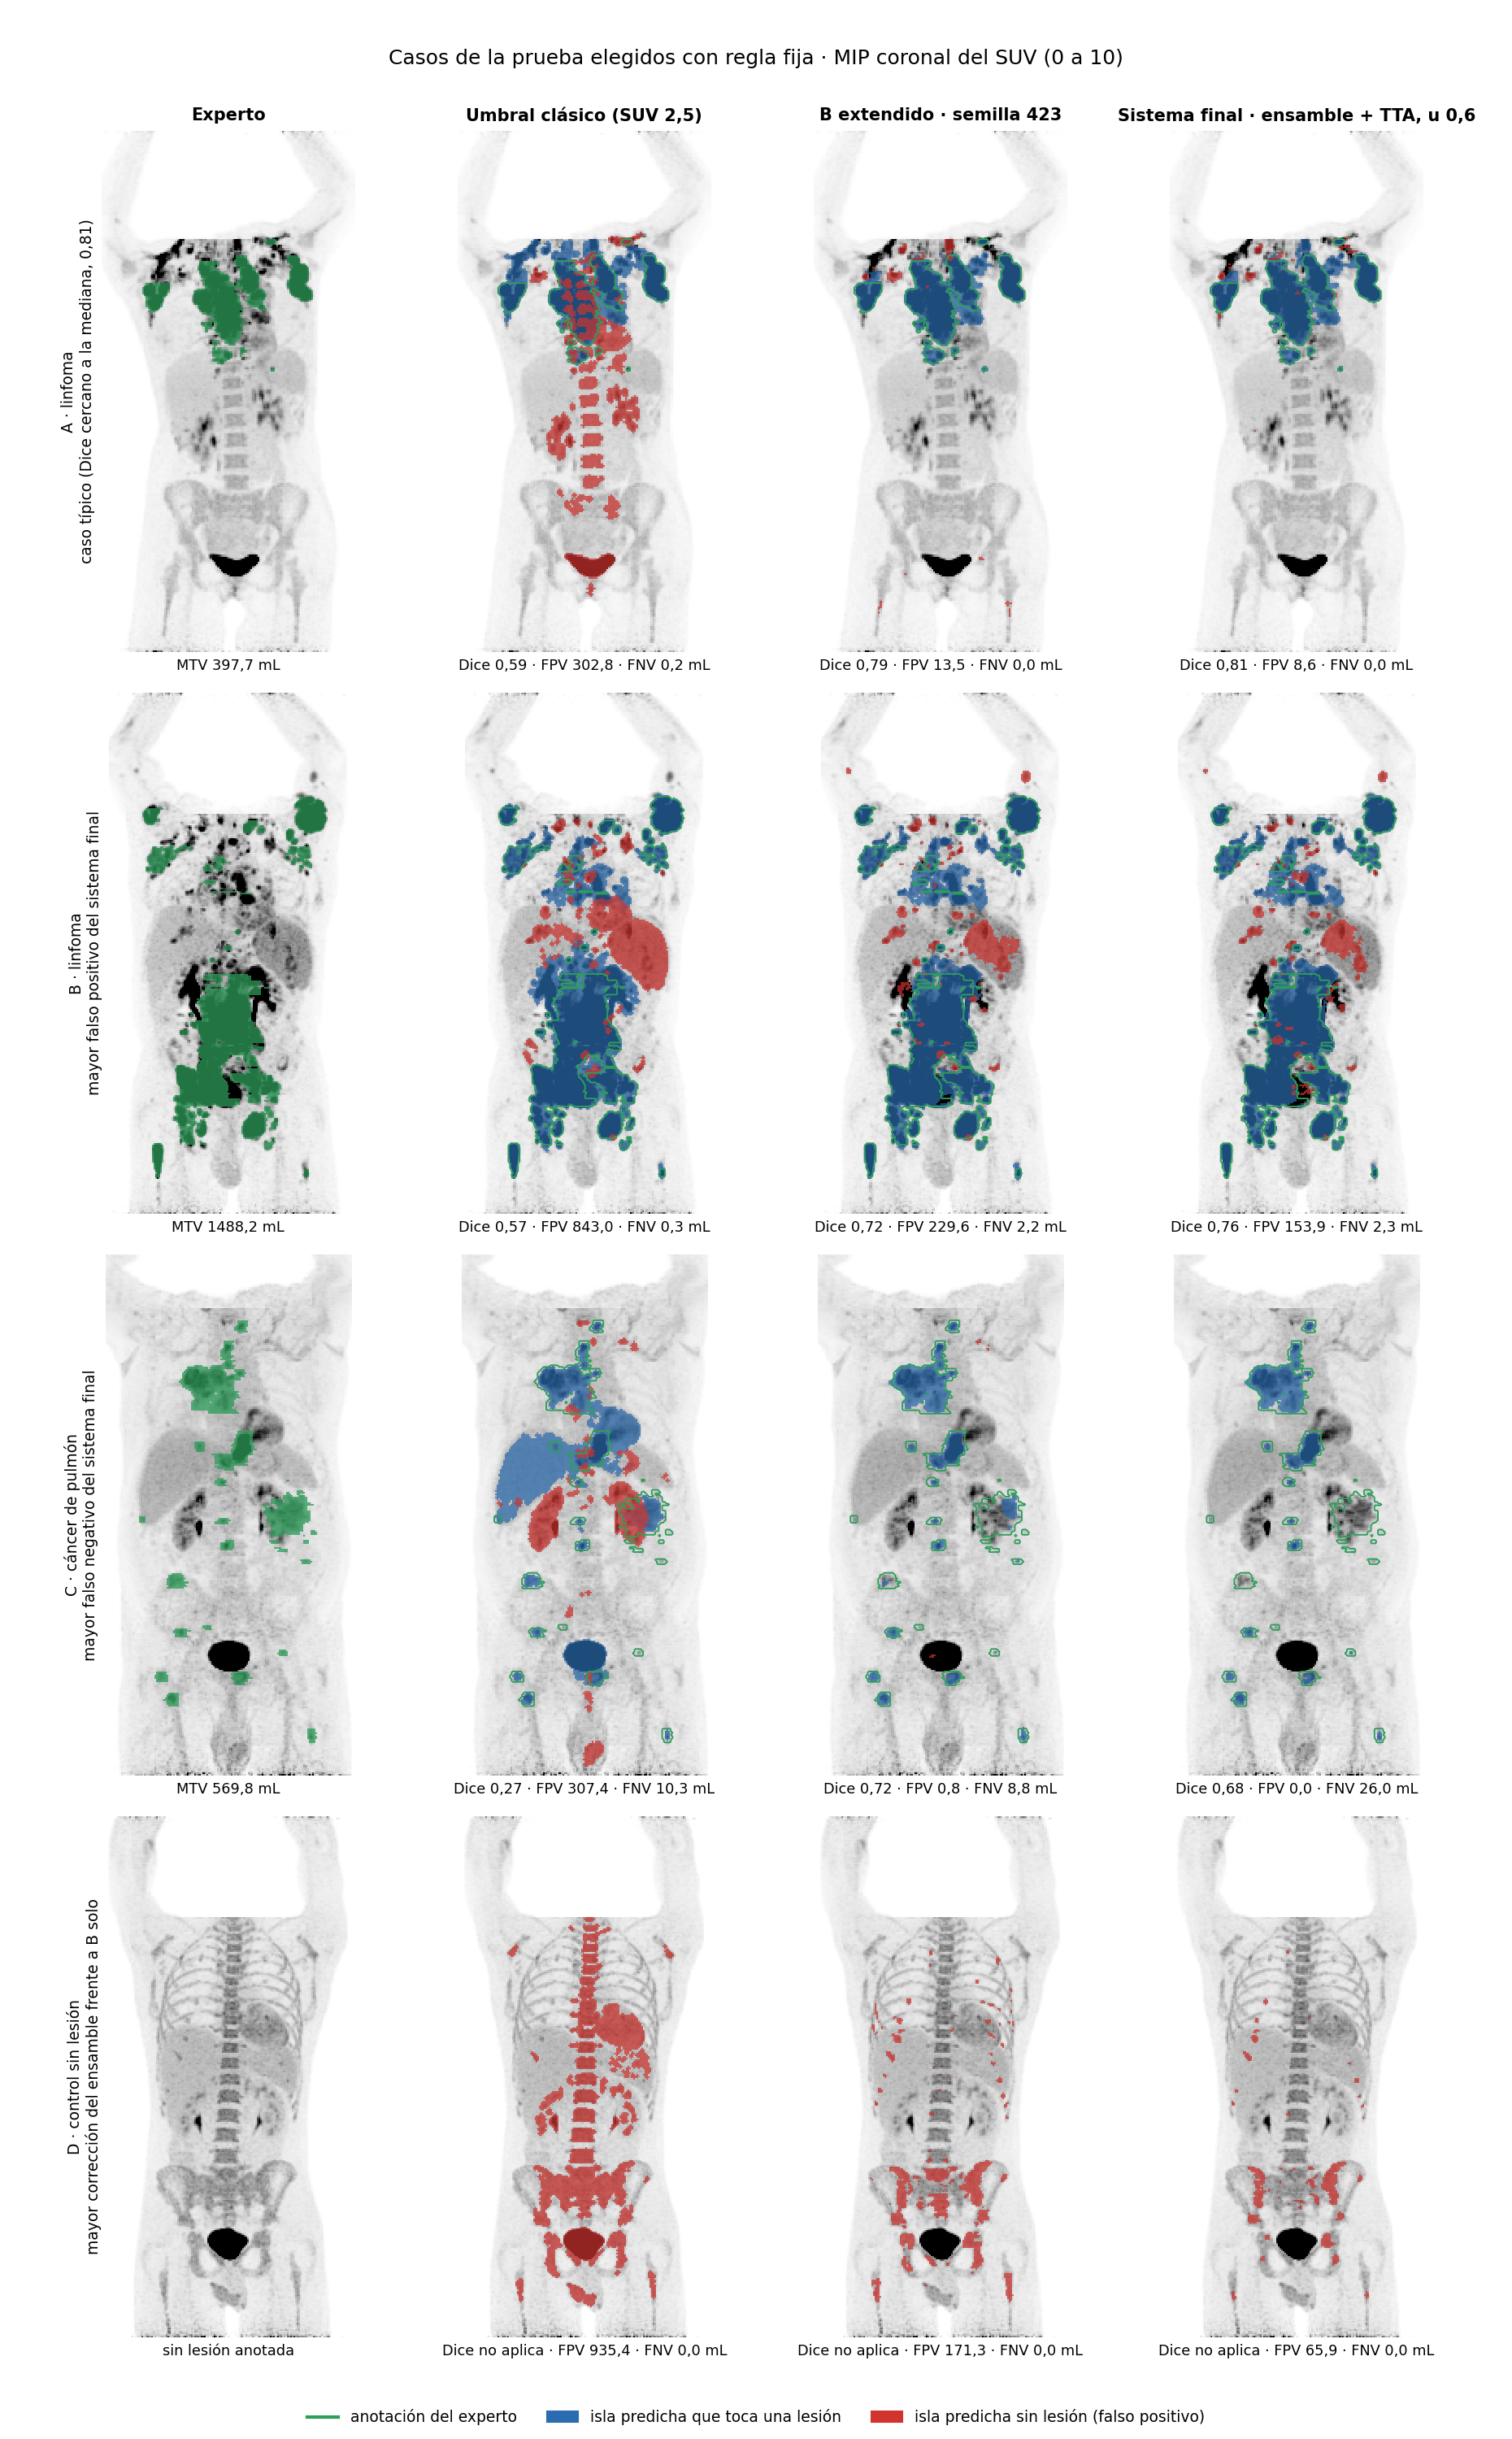
\includegraphics[height=0.86\textheight,keepaspectratio]{casos_test.png}
\caption{Casos de la prueba elegidos con regla fija (\texttt{scripts/42}). MIP coronal del SUV (0 a 10). Verde, anotación del experto; azul, islas predichas que tocan una lesión; rojo, islas predichas sin lesión. Bajo cada panel, las métricas de ese estudio.}
\label{fig:casos}
\end{figure}

\subsection{Análisis secundarios}
\label{sec:secundarios}

Estos análisis estaban comprometidos en la definición de tema pero no en el preregistro de la prueba. Los calculé después de abrirla, sobre las máscaras ya guardadas y sin parámetros ajustables, y no cambian los veredictos de H1 y H2.

\textbf{Hausdorff 95.} En los 38 positivos, la mediana del HD95 es 252,9 mm para la clásica, 93,3 para A del acto 1, 64,1 para B extendido, 31,0 para el ensamble con TTA y 23,5 para el sistema final. Contra B, el sistema final lo baja 16,5 mm (IC95 $-26{,}2$ a $-0{,}7$; mejora en 27 de 38; $p<0{,}001$). Entre arquitecturas no hay diferencia. El HD95 castiga mucho las islas falsas lejanas, y por eso el ensamble, que deja menos marcas falsas, es lo que más lo baja.

\textbf{SUVmax.} En el sistema final el error mediano del SUVmax por paciente es cero y el 87\,\% de los pacientes queda dentro de un 10\,\%, contra 79\,\% de B y 32\,\% de la clásica. De los cinco que quedan fuera, en cuatro la predicción da un SUVmax mayor: marcó algo más caliente que la lesión. Hay dos límites: el preprocesamiento pone tope al SUV en 30, y 4 de los 38 estudios tienen el SUVmax anotado en ese tope; y el SUVmax se mide en la grilla de 3 mm.

\textbf{Script oficial de autoPET.} Sobre las mismas máscaras, en la métrica cruda, el Dice sale idéntico. El oficial cuenta componentes con conectividad 18 y el mío con 26; en las redes, el FPV y el FNV difieren en 3 a 7 de 49 estudios y nunca en más de 0,62 mL. Solo en el umbral clásico, que deja cientos de islas, la diferencia llega a 36 mL en un estudio. Ninguna conclusión cambia.

\textbf{Clásica con exclusión de órganos.} Apagando las islas que caen en más de la mitad dentro de 12 grupos de órganos de captación fisiológica (lista fijada el 24 de septiembre, antes de abrir la prueba), la clásica sube de \dmas{} 0,182 a 0,379 y baja el FPV de 832,5 a 94,8 mL, pero el FNV sube de 2,1 a 28,6 mL porque también apaga metástasis hepáticas y ganglios que el mapa asigna a vasos o corazón. Aun así deja diez veces el FPV del sistema final.

\section{Análisis crítico}

\subsection{Sobre la hipótesis original}

La hipótesis decía que la atención cruzada reduce el FPV frente a la fusión temprana sin aumentar el FNV. En la prueba, la media del FPV de C bajó frente a A del acto 1 y el FNV subió 0,9 mL sin significancia, lo que a primera vista la apoya. Pero B logra lo mismo sin atención, y la ablación de C dio cero. Tal como estaba escrita, la hipótesis no se sostiene en su mecanismo: lo que baja el falso positivo es separar los codificadores, no la atención.

El fracaso de la atención tiene una causa estructural y no de entrenamiento, porque se repitió con $\gamma$ inicial en 0 y en 1, con 25\,000 y con 100\,000 iteraciones, en las siete corridas de C. En el cuello, cada posición resume 48 mm y el CT de todo el parche cabe en 216 posiciones; un promedio de esas posiciones ya describe bien la anatomía general del parche, y eso es lo que la atención aprendió a devolver. La normalización de instancia que viene después borra justamente lo que es igual en todas las posiciones. Para que la anatomía module al PET por esta vía habría que llevar la atención a una resolución mayor, cambiar la normalización o modular la escala y el desplazamiento de la normalización en vez de sumar. Esto no dice que la atención no sirva en PET/CT \citep{fu2021,huang2025,zhao2024}; dice que este diseño concreto no tenía cómo aportar.

\subsection{Por qué se invirtió el orden de las arquitecturas}

Con 25\,000 iteraciones ganaba el modelo chico; con 100\,000, los de doble codificador. Los modelos de 24 M parámetros necesitan más entrenamiento para llegar a su mejor punto, y comparar todo con el mismo presupuesto corto los evaluaba a medio camino. Es el mismo punto que hace la revisión de nnU-Net sobre comparaciones de arquitecturas con entrenamiento insuficiente \citep{isensee2024revisited}: una comparación justa necesita que todos los brazos converjan. El diseño 2\,×\,2 y el control A+ permiten decirlo con evidencia, y no como suposición: el efecto de las iteraciones se repitió en las dos condiciones de datos, y el efecto del tamaño, aislado, fue nulo.

\subsection{Comparación con lo publicado}

El sistema final llega a \dmas{} 0,705 con la métrica cruda del reto y 9,5 mL de FPV. El ganador de autoPET 2022 llegó a 0,623 y 2,84 mL, y la nnU-Net de base a 0,690 y 5,78 mL \citep{gatidis2024challenge,alloula2023}. Esas cifras son de otro conjunto de prueba, con otros pacientes y en parte de otros centros, así que sirven de orientación y no de comparación directa. Con esa salvedad, el Dice está en el rango de lo publicado y el falso positivo sigue siendo entre dos y tres veces mayor. La diferencia principal con nnU-Net que quedó es el aumento de datos: aquí solo hubo volteos, y nnU-Net agrega rotaciones, escalado, ruido y cambios de contraste. También entrena 250\,000 iteraciones por defecto, contra 100\,000 de este trabajo.

\subsection{Lo que aprendí sobre el método}

Tres veces una sola semilla mostró algo que no se repitió: la primera C con 16 mL de FPV, la primera B extendida con +0,033 sobre A y el preentrenamiento con 0,724. Las tres desaparecieron con más semillas. El criterio de checkpoint, a su vez, fabricó la ventaja de E en el acto 1. Por eso todas las comparaciones de este informe usan tres semillas, y las que no las tienen lo dicen. La validación de 26 estudios también engañó con el umbral: decidirlo con los 825 fuera de pliegue evitó llevar a la prueba un umbral de 0,7 que solo era ruido.

\subsection{Fallas que encontré al revisar el trabajo}
\label{sec:fallas}

Antes de cerrar revisé el código y el diseño buscando errores propios. Ninguno de los siguientes cambia las conclusiones de la prueba, pero los declaro porque afectan cómo se leen algunos números.

\begin{itemize}
\item \textbf{Fuga en la validación del acto 1.} La validación rápida que elegía \texttt{mejor.pt} usaba los primeros 12 de los 26 estudios de validación, y la Tabla~\ref{tab:acto1} reporta esos mismos 26. Las cifras de \texttt{mejor.pt} quedan algo optimistas. La columna \texttt{ultimo.pt}, que no pasó por ninguna elección, muestra el mismo empate, y la prueba nunca se usó para elegir nada. Lo correcto habría sido validar durante el entrenamiento con un grupo separado del entrenamiento, no de la validación.
\item \textbf{El factor ``más datos'' del diseño 2\,×\,2 cambió también la proporción de controles}: 20\,\% en los 176 estudios y 50\,\% en los 825. Como en un control los parches se recortan al azar, la fracción de parches centrados en lesión bajó de cerca de 0,56 a 0,35. El efecto de las iteraciones se sostiene, pero el de los datos quedó confundido con ese cambio. Habría que mantener la misma proporción en las dos condiciones.
\item \textbf{Los intervalos no incluyen la variación entre semillas.} El bootstrap remuestrea pacientes sobre el promedio de tres semillas, así que los IC de las comparaciones entre arquitecturas son algo más estrechos de lo que deberían. Un bootstrap jerárquico, que remuestree semillas y pacientes, lo corregiría.
\item \textbf{Las comparaciones secundarias no tienen corrección por multiplicidad.} H1 y H2 están protegidas por el preregistro; S1 a S8 son ocho comparaciones exploratorias, y algunas, como B contra A en el extendido, quedan cerca del límite.
\item \textbf{El ensamble usa 20 veces más cómputo al predecir que B.} Parte de su ventaja viene de ese costo. Una comparación justa sería contra un B con TTA o con el mismo presupuesto de inferencia.
\item \textbf{E solo se entrenó en el acto 1.} Es el único brazo que no se probó con entrenamiento suficiente, así que no sé si con 100\,000 iteraciones habría aportado, como pasó con B.
\item \textbf{La ventana del CT, de $-200$ a 300 HU, deja el pulmón igual que el aire y satura el hueso.} La red pierde anatomía justo en pulmón y hueso, donde queda parte del falso positivo. Una ventana más amplia o dos canales de CT con ventanas distintas lo evitarían.
\end{itemize}

\subsection{Limitaciones}

\begin{itemize}
\item \textbf{Un solo centro y una sola anotación.} autoPET viene de un hospital y cada estudio tiene un anotador. No hay medida de variabilidad entre expertos.
\item \textbf{La anotación no marca inflamación.} Cuando una red marca un ganglio del mediastino en un control, no se puede saber si es error o un hallazgo no anotado. Evité las preguntas que la anotación no puede contestar.
\item \textbf{Zona anonimizada excluida.} El trabajo no dice nada sobre cabeza, cuello ni encéfalo.
\item \textbf{Resolución de 3 mm y tope de SUV en 30.} Las lesiones de menos de 1 mL tienen pocos vóxeles, y el SUVmax de cuatro estudios queda truncado.
\item \textbf{Métricas propias}, contrastadas con el script oficial con diferencias menores a 1 mL en las redes.
\item \textbf{La MTV automática no sirve todavía para seguimiento} en pacientes de carga alta: en el acto 1 los límites de concordancia fueron de $-244$ a $+184$ mL.
\item \textbf{El umbral se decidió fuera de pliegue}, con un solo miembro del ensamble por estudio, que es un sustituto del ensamble completo.
\end{itemize}

\section{Conclusiones y trabajo futuro}

\begin{enumerate}
\item Las redes le ganan al umbral clásico por un margen enorme, y le ganan justo donde el umbral no sabe anatomía: en los órganos de captación fisiológica, donde dejan menos de 1 mL por estudio.
\item Separar los codificadores del PET y del CT mejora la segmentación cuando la red entrena lo suficiente, en Dice y en falso positivo, y no por tener más parámetros. Con poco entrenamiento la comparación sale empatada o al revés.
\item La atención cruzada aditiva en el cuello de una U-Net con normalización de instancia no aporta nada, y se conoce el mecanismo.
\item Enseñar anatomía de forma explícita, con preentrenamiento o con una pérdida pesada por órgano, no cambió el resultado.
\item El ensamble de cinco pliegues con TTA es la mejora más grande y más sólida. El sistema final, decidido sin mirar la prueba, quedó en \dmas{} 0,727 y 9,5 mL de FPV.
\item Hay hallazgos de método que valen por sí mismos: el criterio de checkpoint puede fabricar diferencias, el presupuesto de entrenamiento puede invertir el orden de las arquitecturas y una semilla sola no basta para afirmar nada.
\end{enumerate}

\textbf{Trabajo futuro.} Lo más directo es probar la atención a mayor resolución o como modulación de la normalización, siempre con su ablación y su control de capacidad. También quedan el aumento de datos completo de nnU-Net y más iteraciones, que es la diferencia principal con lo publicado. En lo clínico, la extensión natural es medir el trabajo real de corrección de un médico sobre la máscara propuesta y validar en otro centro, por ejemplo con los datos multitrazador de autoPET III \citep{gatidis2026autopet3}.


\sloppy
\small
\bibliographystyle{unsrtnat}
\bibliography{referencias}
\normalsize

\section*{Declaración de uso de inteligencia artificial}
{\small
Usé Claude (Anthropic) como asistente durante el proyecto: para revisar y depurar código, proponer la estructura de algunos scripts, discutir alternativas de diseño y corregir la redacción de este informe. Las decisiones del trabajo son mías: la pregunta, el diseño experimental, la elección de datos y métricas, la ejecución de los entrenamientos, la lectura de los resultados y las conclusiones. Revisé cada número de este informe contra las tablas del repositorio y respondo por todo lo que aquí se afirma.\par}


\end{document}

